\section*{Preface: Bridging Text between Chapters 2 and 3}
\addcontentsline{toc}{section}{Preface: Bridging Text between Chapters 2 and 3}


In this chapter, the population-based approach used to detect arm-level CNV was extended to the detection of small CNV across the genome.
Instead of testing one chromosomal arm at a time, the genome is tiled and each region is tested for CNV using the same strategy: a set of reference samples is used to deal with technical variation.
By better integrating technical variation, our goal is to improve the robustness and sensitivity of the CNV detection.
Notably, this chapter introduces {\sf PopSV}, the CNV detection method implemented in the context of this thesis, and its application to a disease study.
{\sf PopSV} is later used in chapter \ref{chap:rep} to investigate CNVs in low-mappability regions.

In this Research Article published in {\it PLoS Genetics}\cite{Monlong2018}, we first introduce the rationale for the method: the presence of visible technical bias in WGS coverage data.
After an overview of the method, we show that it is more sensitive than other methods and avoids systematic calls.
Finally, we apply {\sf PopSV} to WGS data from 198 epilepsy patients and 301 controls and show CNV enrichments in exons and non-coding regions that potentially explain an important fraction of patients.
\nameref{append:epi} contains supplementary tables, figures and information.
\bigskip

\newpage
\singlespacing

\begin{center}
  \LARGE\bf Global characterization of copy number variants in epilepsy patients from whole genome sequencing
\end{center}
\bigskip

\large{Jean Monlong$^{1,2,*}$, Simon L. Girard$^{1,3,4,*}$, Caroline Meloche$^{4}$, Maxime Cadieux-Dion$^{4,5}$, Danielle M. Andrade$^{6}$, Ron G. Lafreniere$^{4}$, Micheline Gravel$^{4}$, Dan Spiegelman$^{7}$, Alexandre Dionne-Laporte$^{7}$, Cyrus Boelman$^{8}$, Fadi F. Hamdan$^{9}$, Jacques L. Michaud$^{9}$, Guy Rouleau$^{7}$, Berge A. Minassian$^{10}$, Guillaume Bourque$^{1,2,11,+}$, Patrick Cossette$^{4,+}$}
\bigskip

\footnotesize
$^{1}$ Department of Human Genetics, McGill University, Montr\'eal, H3A 1B1, Canada

$^{2}$ Canadian Center for Computational Genomics, Montr\'eal, H3A 1A4, Canada

$^{3}$ D\'epartement des sciences fondamentales, Universit\'e du Qu\'ebec \`a  Chicoutimi, Chicoutimi, G7H 2B1, Canada

$^{4}$ Centre de Recherche du Centre Hospitalier de l'Universit\'e de Montr\'eal, Montr\'eal, H2X 0A9, Canada

$^{5}$ Center for Pediatric Genomic Medicine, Children's Mercy Hospital, Kansas City, MO, USA

$^{6}$ Epilepsy Genetics Program, Division of Neurology, Toronto Western Hospital, University of Toronto, Toronto, Canada

$^{7}$ Montreal Neurological Institute, McGill University, Montr\'eal, H3A 2B4, Canada

$^{8}$ Division of Neurology, BC Children's Hospital, Vancouver, V6H 3N1, Canada

$^{9}$ CHU Sainte-Justine Research Center, Montr\'eal, H3T 1C5, Canada

$^{10}$ Division of Neurology, The Hospital for Sick Children, Toronto, M5G 1X8, Canada

$^{11}$ McGill University and G\'enome Qu\'ebec Innovation Center, Montr\'eal, H3A 1A4, Canada

$^+$Correspondence: guil.bourque@mcgill.ca or patrick.cossette@umontreal.ca

$^*$These authors contributed equally to this work


\normalsize
\doublespacing

\section{Abstract}
Epilepsy will affect nearly 3\% of people at some point during their lifetime. 
Previous copy number variants (CNVs) studies of epilepsy have used array-based technology and were restricted to the detection of large or exonic events. 
In contrast, whole-genome sequencing (WGS) has the potential to more comprehensively profile CNVs but existing analytic methods suffer from limited accuracy. 
We show that this is in part due to the non-uniformity of read coverage, even after intra-sample normalization. 
To improve on this, we developed {\sf PopSV}, an algorithm that uses multiple samples to control for technical variation and enables the robust detection of CNVs. 
Using WGS and {\sf PopSV}, we performed a comprehensive characterization of CNVs in 198 individuals affected with epilepsy and 301 controls. 
For both large and small variants, we found an enrichment of rare exonic events in epilepsy patients, especially in genes with predicted loss-of-function intolerance. 
Notably, this genome-wide survey also revealed an enrichment of rare non-coding CNVs near previously known epilepsy genes. 
This enrichment was strongest for non-coding CNVs located within 100 Kbp of an epilepsy gene and in regions associated with changes in the gene expression, such as expression QTLs or DNase I hypersensitive sites. 
Finally, we report on 21 potentially damaging events that could be associated with known or new candidate epilepsy genes. 
Our results suggest that comprehensive sequence-based profiling of CNVs could help explain a larger fraction of epilepsy cases. 


\section{Author Summary}
Epilepsy is a common neurological disorder affecting around 3\% of the population.
In some cases, epilepsy is caused by brain trauma or other brain anomalies but there are often no clear causes.
Genetic factors have been associated with epilepsy in the past such as rare genetic variations found by linkage studies as well as common genetic variations found by genome-wide association studies and large copy-number variants.
We sequenced the genome of $\sim$200 epilepsy patients and $\sim$300 healthy controls and compared the distribution of deletion (loss of a copy) and duplication (additional copy) of genomic regions.
Thanks to the sequencing technology and a new method that takes advantage of the large sample size, we could compare the distribution of small copy-number variants between epilepsy patients and controls.
Overall, we found that small variants are also associated with epilepsy.
Indeed, the genome of epilepsy patients had more exonic copy-number variants, especially when rare or affecting genes with predicted loss-of-function intolerance.
Focusing on regions around genes that have been previously associated with epilepsy, we also found more non-coding variants in epilepsy patients, especially deletions or variants in regulatory regions.
Finally, we provide a list of 21 regions in which we found likely pathogenic variants.

\section{Introduction}
Structural variants (SVs) are defined as genetic mutations affecting more than 50 base pairs and encompass several types of rearrangements: deletion, duplication, novel insertion, inversion and translocation.
Deletions and duplications, which affect DNA copy number, are collectively known as copy number variants (CNVs).
SVs arise from a broad range of mechanisms and show a heterogeneous distribution of location and size across the genome\cite{Hall2012,Sharp2006,Mills2011}.
Numerous diseases are caused by SVs with a demonstrated detrimental effect\cite{Conrad2010,Spielmann2013}.
While cytogenetic approaches and array-based technologies have been used to identify large SVs, whole-genome sequencing (WGS) has the potential to uncover the full range of SVs both in terms of type and size\cite{Zhao2013a,Pirooznia2015}.
SV detection methods that use read-pair and split read information\cite{Layer2012} can detect deletions and duplications but most CNV-focused approaches look for an increased or decreased read coverage, the expected consequence of a duplication or a deletion.
Coverage-based methods exist to analyze single samples\cite{Abyzov2011}, pairs of samples\cite{Boeva2011} or multiple samples\cite{Handsaker2015,Klambauer2012,Glusman2015} but the presence of technical bias in WGS remains an important challenge.
Indeed, various features of sequencing experiments, such as mappability\cite{Treangen2011,Teo2012}, GC content\cite{Benjamini2012}, replication timing\cite{Koren2014}, DNA quality and library preparation\cite{VanDijk2014}, have a negative impact on the uniformity of the read coverage\cite{Cheung2011}.

Epilepsy is a common neurological disorder characterized by recurrent and unprovoked seizures.
It is estimated that up to 3\% of the population will suffer from a form of epilepsy at some point during their lifetime.
Although the disease presents a strong genetic component that can be as high as 95\%, typical ``monogenic'' epilepsy is rare, accounting for only a fraction of cases\cite{Berkovic1998,Zara1995}.
Genetic factors have been associated with epilepsy in the past such as rare genetic variations found by linkage studies as well as common genetic variations found by genome-wide association studies\cite{Kasperaviciute2010a,Guo2012}
For example, a meta-analysis combining multiple epilepsy cohorts found positive associations with the disease\cite{InternationalLeagueAgainstEpilepsyConsortiumonComplexEpilepsies2014}, the strongest in {\it SCN1A}, a gene already associated with the genetic mechanism of the disease via linkage studies and subsequent sequencing\cite{Escayg2000} or more recently as harboring {\it de novo} variants\cite{Claes2003}.
Thanks to array-based technologies, surveys of large CNVs ($>$50 Kbp) first associated CNVs in genomic hotspots such as 15q11.2 and 16p13.11 with generalized epilepsy\cite{Helbig2009,DeKovel2010}.
Other studies have further shown the importance of large and \textit{de novo} CNVs as well as identified a few associations with specific genes\cite{Mefford2010,Helbig2014,Mefford2015,Addis2016,Biervert1998,Lal2015}.
Rare genic CNVs were typically found in around 10\% of epilepsy patients\cite{Mefford2011,Mefford2010,Addis2016} and CNVs larger than 1 Mbp were significantly enriched in patients compared to controls\cite{Mefford2011,Heinzen2010,Striano2012,Lal2015}.
Unfortunately, small CNVs and other types of SVs could not be efficiently or consistently detected using these technologies, hence much remains to be done.

To more comprehensively characterize the role of CNVs in epilepsy, we performed whole-genome sequencing of epileptic patients from the Canadian Epilepsy Network (CENet), the largest WGS study on epilepsy to date.
In the present study, we assessed the frequency of CNVs in epileptic individuals using 198 unrelated patients and 301 healthy individuals. Using this data, we showed that technical variation in WGS remains problematic for CNV detection despite state-of-the-art intra-sample normalization.
To correct for this and to maximize the potential of the CENet cohorts, we developed a population-based CNV detection algorithm called {\sf PopSV}.
Our method uses information across samples to avoid systematic biases and to more precisely detect regions with abnormal coverage.
Using two public WGS datasets\cite{Scelo2014,Boivin2013}, and additional orthogonal validation, we showed that {\sf PopSV} outperforms other analytical methods both in terms of specificity and sensitivity, especially for small CNVs.
Using this tool, we built a comprehensive catalog of CNVs in the CENet epilepsy patients and studied the properties of these potentially damaging structural events across the genome.


\section{Results}

\subsection*{Technical bias in read coverage}
We sequenced the genomes of 198 unrelated individuals affected with epilepsy and 301 unrelated healthy controls.
Because CNV detection relies on read coverage we first investigated the presence of technical bias and the value of standard corrections and filters (e.g. GC correction, mappability filtering).
The genome was fragmented in 5 Kb bins and we counted the number of uniquely mapped reads in each bin.
In contrast to simulated datasets, we found that the inter-sample mean coverage in each bin varied between genomic regions even after stringent corrections and filters (Fig. \ref{fig:wgsbias}).
Supporting this observation, the bin coverage variance across samples was also lower than expected and varied between regions (Fig. \ref{fig:bias:var}).
We also observed experiment-specific biases. In particular, some samples consistently had the highest, or the lowest, coverage across large portions of the genome (Fig. \ref{fig:bias:rank}).
These observations were not unique to our data and could also be observed in two public WGS datasets, and persisted even after correcting the GC bias and mappability using the more elaborate model from the {\sf QDNAseq} pipeline\cite{Scheinin2014} (Fig. \ref{fig:wgsbias2}).
Our results across multiple samples suggest that existing GC bias and mappability corrections\cite{Scheinin2014} cannot correct completely the technical variation in read coverage.
This fluctuation of coverage has implications for CNV detection approaches that assume a uniform distribution\cite{Boeva2011,Abyzov2011,Xi2011} after standard bias correction and will lead to false positives.

\begin{figure}[!h]
  \begin{subfigure}[b]{.3\linewidth}
    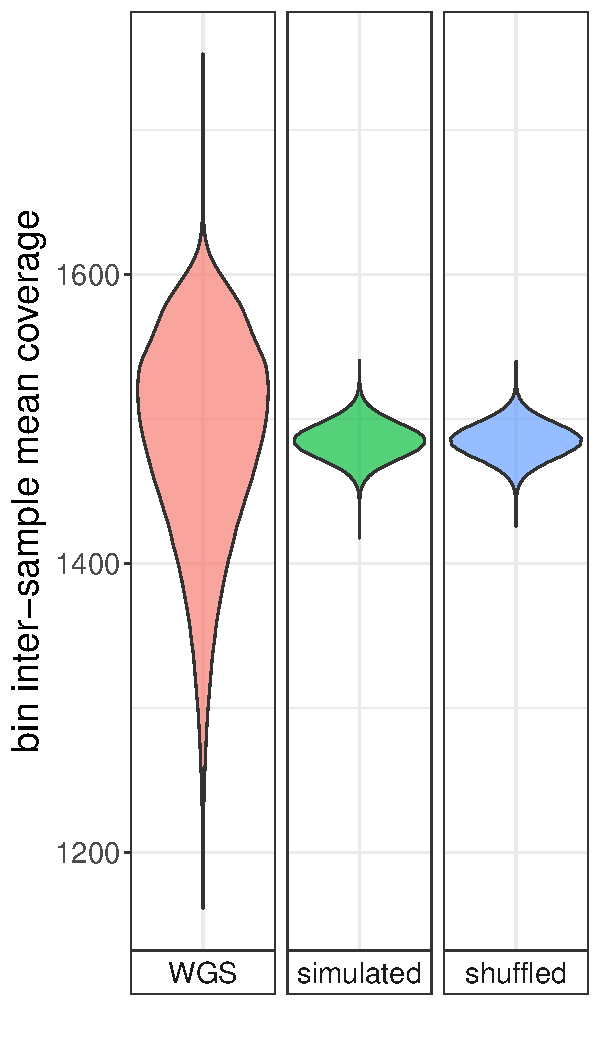
\includegraphics[width=\linewidth,page=1]{figures/epilepsy-biasWGS-thin.pdf}
    \caption{}
    \label{fig:wgsbias}
  \end{subfigure}
  \unskip\ \vrule\
  \begin{subfigure}[b]{.7\linewidth}
    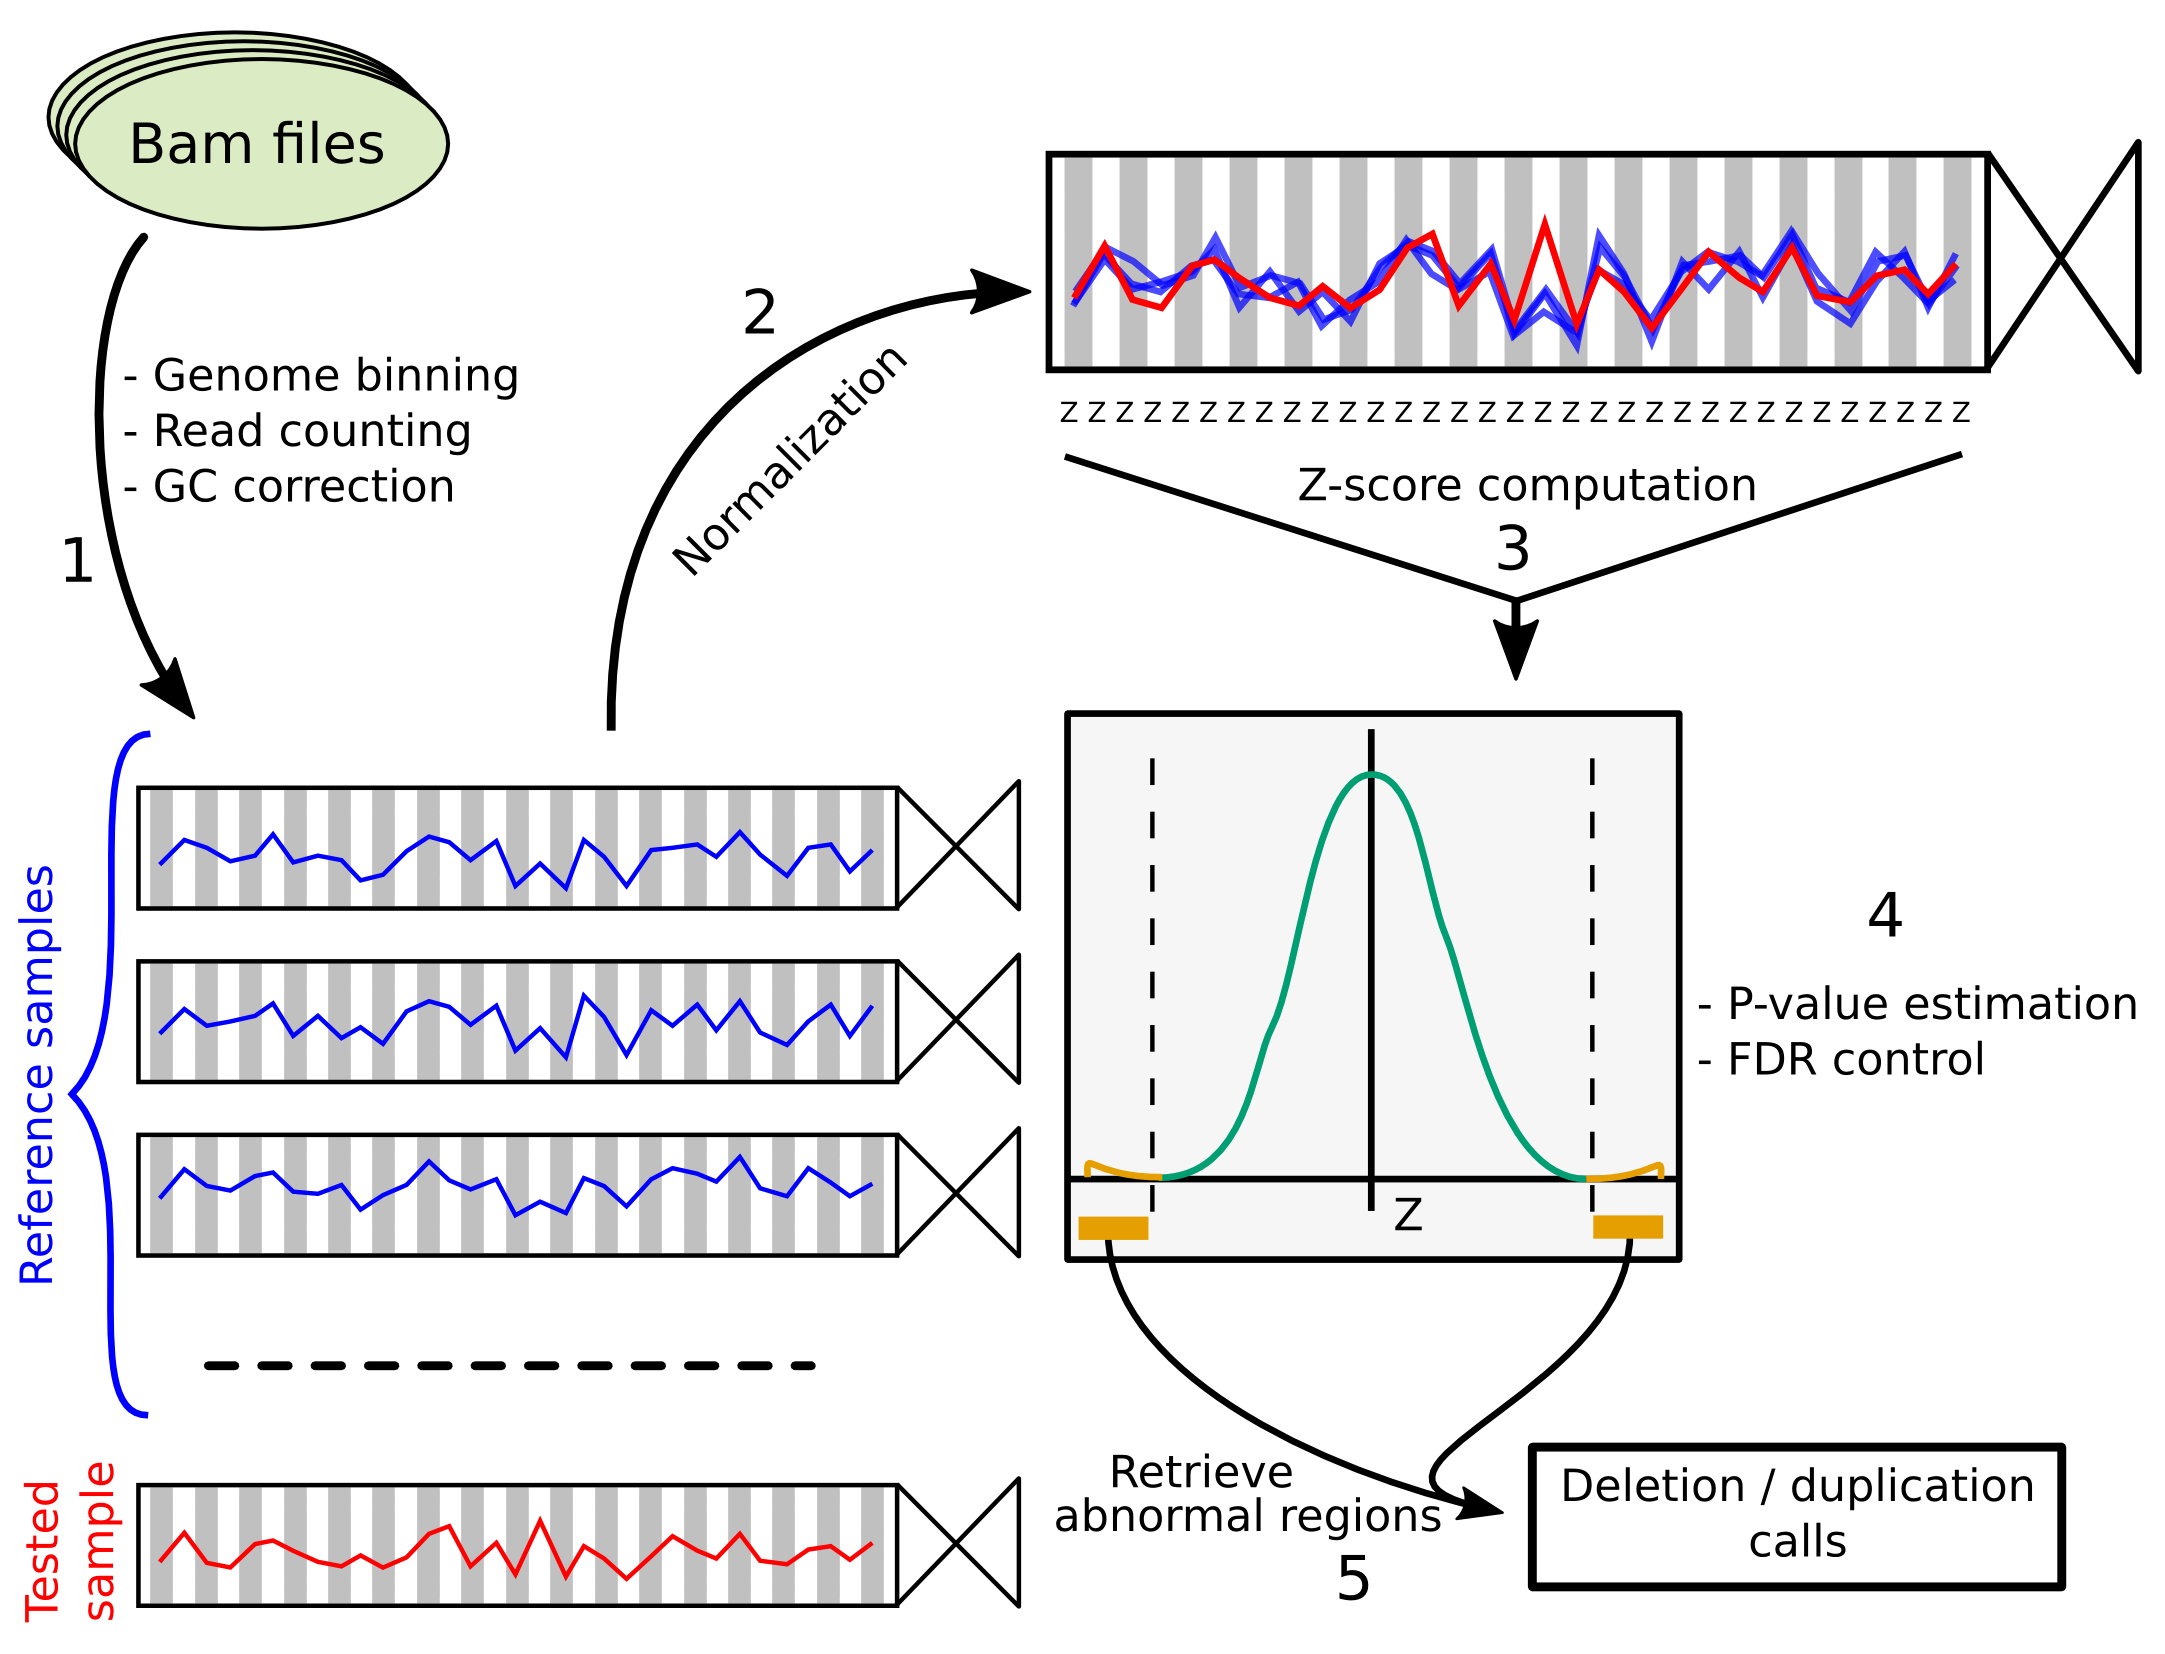
\includegraphics[width=\linewidth]{figures/PopSVworkflow.png}
    \caption{}
    \label{fig:popsv}
  \end{subfigure}
  \unskip \hrule\
  \medskip

  \begin{subfigure}[b]{\linewidth}
    \includegraphics[width=.5\linewidth, page=2]{figures/twin-benchmark-long.pdf}
    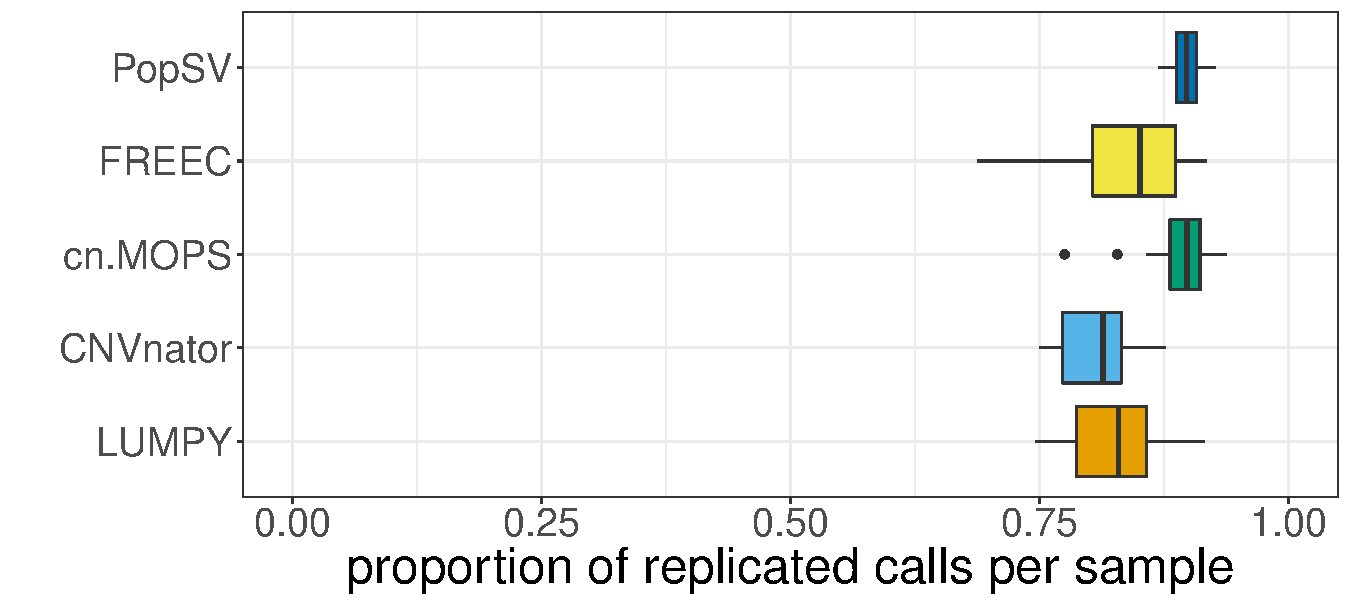
\includegraphics[width=.5\linewidth, page=1]{figures/twin-benchmark-long.pdf}
    \caption{}
    \label{fig:twinconc}
  \end{subfigure}
  \caption[{\sf PopSV} approach]{{\bf {\sf PopSV} approach. } {\small a) Technical bias across the genome remains after stringent correction and filtering. The distribution of the bin inter-sample mean coverage in the epilepsy cohort (red) is compared to null distributions (blue: bins shuffled, green: simulated normal distribution). b) {\sf PopSV} approach. First the genome is fragmented and reads mapping in each bin are counted for each sample and GC corrected (1). Next, coverage of the sample is normalized (2) and each bin is tested by computing a Z-score (3), estimating p-values (4) and identifying abnormal regions (5). c) Number and proportion of calls from a twin that was replicated in the other monozygotic twin.}}
\end{figure}


\subsection*{CNV detection with {\sf PopSV}}
To better control for technical bias, we developed {\sf PopSV}, a new SV detection method.
{\sf PopSV} uses read depth across the samples to normalize coverage and detect change in DNA copy number (Fig. \ref{fig:popsv}).
The normalization step here is critical since most approaches will fail to give acceptable normalized coverage scores (Fig. \ref{fig:bias:rank}).
Moreover, with global median/variance adjustment or quantile normalization, the remaining subtle experimental variation impairs the abnormal coverage test (Fig. \ref{fig:zscoreEx:worstZ}).
The targeted normalization used by {\sf PopSV} was found to have better statistical properties (Fig. \ref{fig:normComp}).
In order to assess the performance of our tool, we compared it to several algorithms\cite{Boeva2011,Abyzov2011,Klambauer2012,Layer2012} using a dataset that included monozygotic twins and also performed experimental validation of different types of predicted CNVs in the epilepsy cohort (see below).
We found that {\sf PopSV} performed as well or better in different aspects.
First, for several algorithms, a large proportion of the detected events in a typical sample were also identified in almost all samples (60\% of the calls found in $>$95\% of the samples, Fig. \ref{fig:freqmeth}).
{\sf PopSV}'s calls were better distributed across the frequency spectrum, hence more informative as we expect the relative frequency of disease-related variants to be rare.
In addition, the pedigree structure was more accurately recovered when the CNVs were used to cluster the individuals in the Twins dataset (Fig. \ref{fig:twinclust}).
The agreement with the pedigree was computed by the Rand index after clustering the individuals with three hierarchical clustering approaches (see \nameref{sec:suppmat:epipopsv}).
Looking at the replication between 10 pairs of monozygotic twins, {\sf PopSV} detected more replicated CNVs compared to other methods, while maintaining similar replication rates (Fig. \ref{fig:twinconc}).
The CNV calls were further filtered with gradually more stringent significance thresholds and {\sf PopSV} remained superior in term of number of replicated calls (Fig. \ref{fig:twinconcsig}).
When investigating the overlap of calls between different methods, we noticed that {\sf PopSV} was better recovering calls from {\sf CNVnator}\cite{Abyzov2011}, {\sf FREEC}\cite{Boeva2011}, {\sf cn.MOPS}\cite{Klambauer2012} or {\sf LUMPY}\cite{Layer2012}, especially if found by two or more methods (Fig. \ref{fig:twincallcomp}).
For example, around 92\% of the CNVs called by other methods were also found by {\sf PopSV} when focusing on calls found in at least two methods.
Similar results were also obtained in a cancer dataset where we looked for replicated germline CNVs in the paired tumor (Fig. \ref{fig:ckconc}).
Finally, we repeated the twin analysis using 500 bp bins and observed high consistency with the 5 Kbp calls (Fig. \ref{fig:compsize}).
These results suggest that {\sf PopSV} can accurately detect around 75\% of events that are as large as half the bin size used (see \nameref{sec:suppmat:epipopsv}).

\subsection*{CNVs in the CENet cohorts and experimental validation}
Having demonstrated the quality of the {\sf PopSV} calls, we applied our tool to the epilepsy and control cohorts.
The epilepsy cohort comprises 198 individuals diagnosed with either generalized (n=160), focal (n=32) or unclassified (n=6) epilepsy.
CNVs ranged from 5 Kbp to 3.2 Mbp with an average size of 9.98 Kbp.
We observed an average of 870 CNVs per individual accounting for 8.7 Mb of variant calls (Fig. \ref{fig:cnvs}).
This is around 9 times more variants and considerably smaller than in typical array-based studies\cite{Redon2006,Itsara2009}, such as the previous epilepsy surveys\cite{Mefford2011,Mefford2010,Helbig2014,Addis2016}, although a similar size distribution was previously obtained using denser arrays\cite{Conrad2010} but were never applied to epilepsy (Fig. \ref{fig:arraysize}).
Next, we annotated each variant using four public SV databases\cite{Sudmant2015a,Handsaker2015,Francioli2014,Sudmant2015} as well as an internal database of the germline calls from {\sf PopSV} in the two public datasets used earlier (see \nameref{sec:suppmat:epipopsv}).
For each CNV, we derived the maximum frequency across these databases and defined as rare any region consistently annotated in less than 1\% of the individuals (Fig. \ref{fig:cnvfreq}).
In total, we identified 12,480 regions with rare CNVs in the epilepsy cohort including: 8,022 (64.3\%) with heterozygous deletions, 21 (0.2\%) with homozygous deletions and 4,850 (38.9\%) with duplications.
Although the overall amount of rare CNVs was not higher in epilepsy patients, the proportion of deletion was significantly higher compared to controls ($\chi^2$ test: P-value $10^{-7}$).
Next, we selected 151 CNVs and further validated them using a Taqman CNV assay and Real-Time PCR.
To explore {\sf PopSV}'s performance across different CNV profiles, we selected variants of different types, sizes and frequencies.
We found that the calls were concordant in 90.7\% of the cases (Table \ref{tab:validationrates} and \ref{tab:validation}).
As expected, the estimated false positive rate was slightly higher for rare or smaller variants (12.1\% for rare CNVs; 15.1\% for CNV $<$20 Kbp).
Furthermore, we noted that calls supported by both {\sf PopSV} and {\sf LUMPY} (when available) had a similar validation rate as calls found by {\sf PopSV} only (86.2\% and 87.5\% respectively).

\begin{figure}[!h]
  \centering
  \begin{subfigure}[b]{.49\textwidth}
    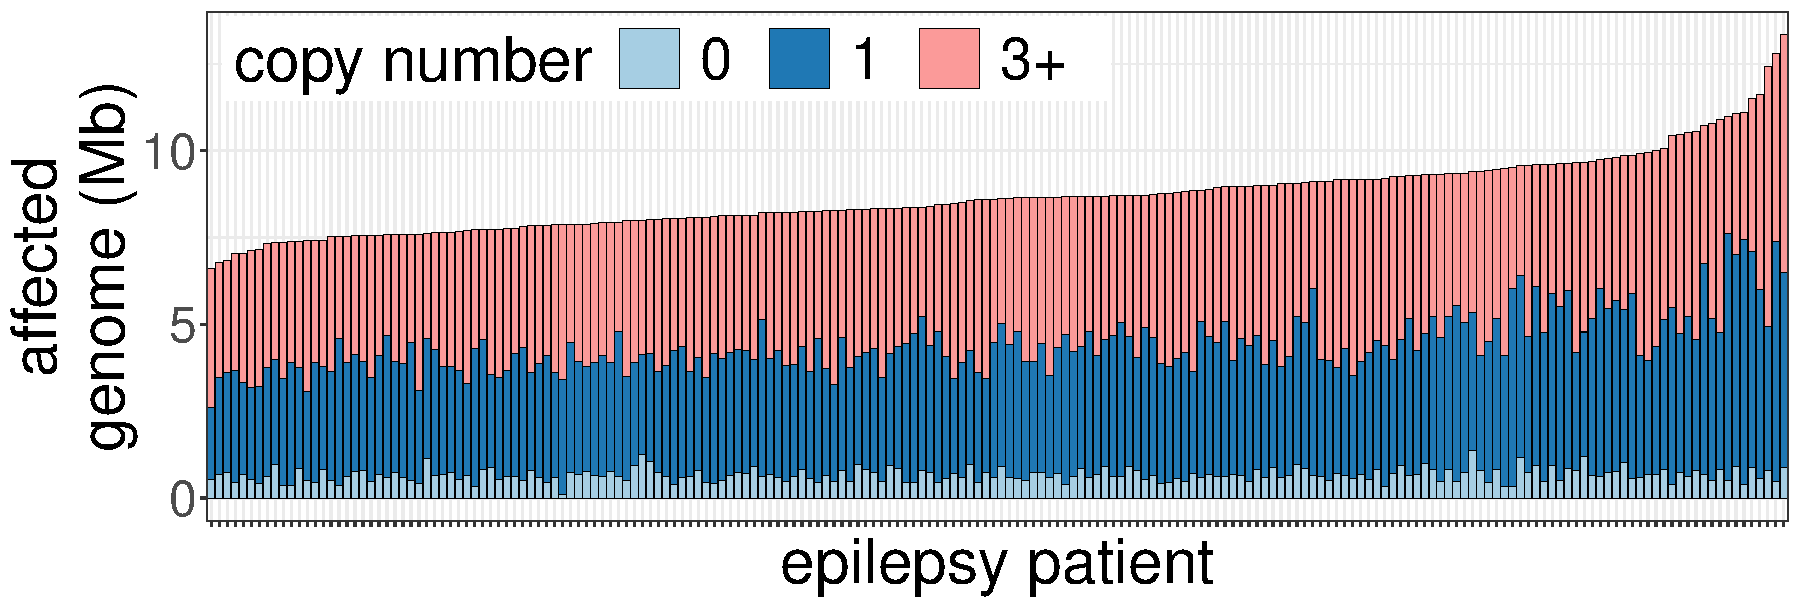
\includegraphics[width=\linewidth, page=1]{figures/epilepsy-CNVnumbers.pdf}
    \caption{}
    \label{fig:cnvs}
  \end{subfigure}
  \begin{subfigure}[b]{.49\textwidth}
    \includegraphics[width=\linewidth, page=3]{figures/epilepsy-CNVnumbers.pdf}
    \caption{}
    \label{fig:cnvfreq}
  \end{subfigure}
  \medskip
  
  \begin{subfigure}[b]{.9\textwidth}
    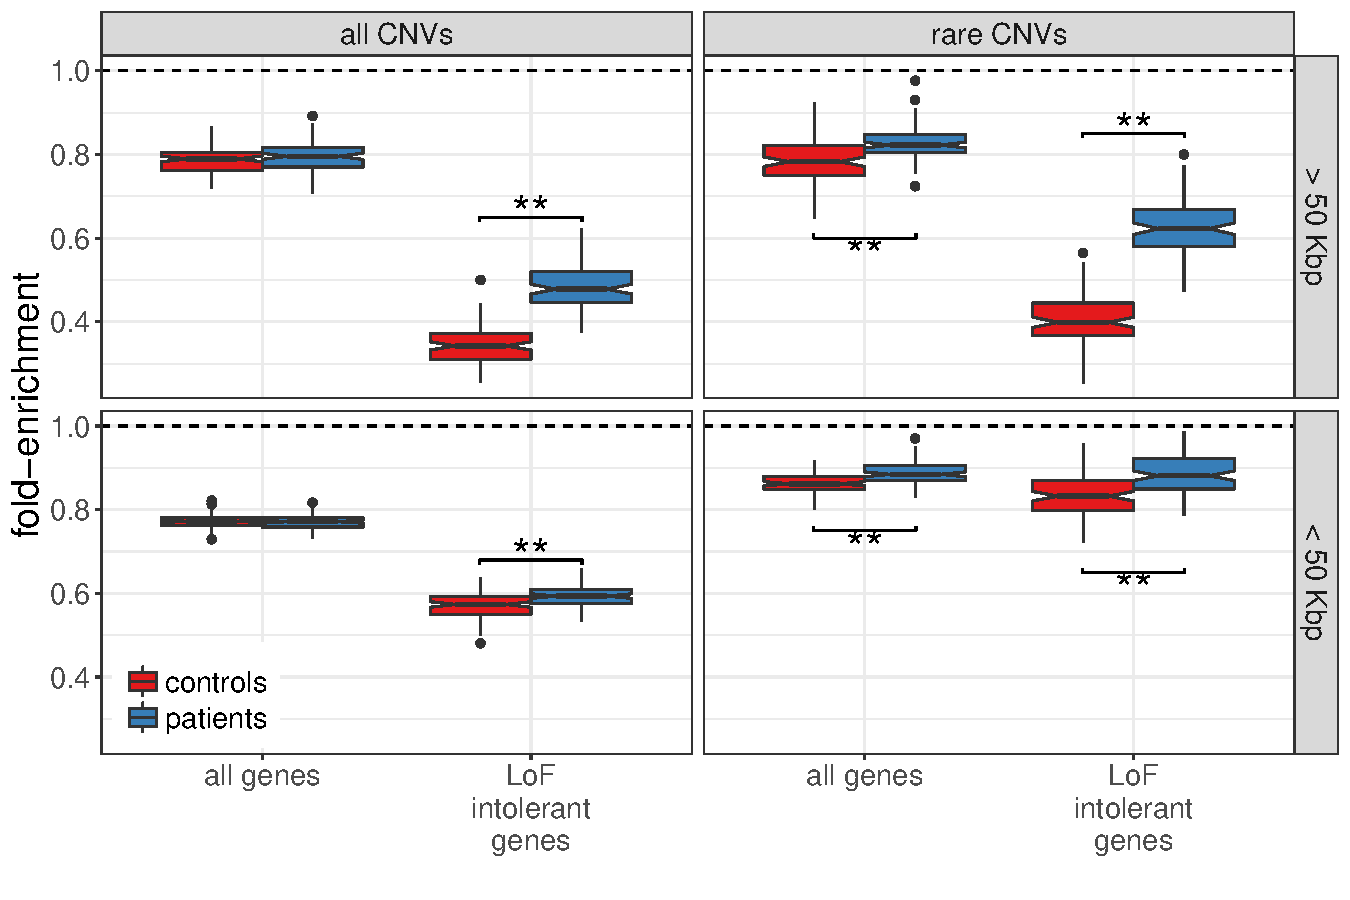
\includegraphics[width=\linewidth,page=1]{figures/epilepsy-enrichmentPatterns.pdf}
    \caption{}
    \label{fig:exenr}
  \end{subfigure}
  \caption[CNVs in the epilepsy and control cohorts.]{{\bf CNVs in the epilepsy and control cohorts.} {\small a) Regions with a CNV in each epilepsy patient. b) Each CNV in the CNV catalog of the epilepsy and control cohorts was annotated with its maximum frequency in five CNV databases. c) Enrichment in exonic sequence for all CNVs (left) and rare CNVs (right), larger than 50 Kbp (top) or smaller than 50 Kbp (bottom). The fold-enrichment (y-axis) represents how many CNVs overlap coding sequences compared to control regions randomly distributed in the genome.}}
\end{figure}

\begin{table}[!ht]
  \renewcommand{\arraystretch}{.7}
  \centering
  \caption[Real-Time PCR validation rates of {\sf PopSV} calls.]{{\bf Real-Time PCR validation rates of {\sf PopSV} calls.}}
  \begin{tabular}[c]{|l|r|r|}
    \hline
                            & Region & Validation rate \\
    \hline
    Total                   & 151    & 0.907           \\
    \hline
    CNV type                &        &                 \\
    $~~$Deletion            & 102    & 0.902           \\
    $~~$Duplication         & 49     & 0.918           \\
    \hline
    Frequency in databases   &        &                 \\
    $~~0$                   & 26     & 0.923           \\
    $~~(0,0.01]$            & 24     & 0.833           \\
    $~~(0.01,1]$            & 101    & 0.921           \\
    \hline
    Carrier in CENet cohorts&        &                 \\
    $~~1$                   & 21     & 0.857           \\
    $~~2$                   & 19     & 0.947           \\
    $~~>2$                  & 111    & 0.910           \\
    \hline
    Size (Kbp)              &        &                 \\
    $~~<20$                 & 73     & 0.849           \\
    $~~(20,100]$            & 38     & 0.974           \\
    $~~>100$                & 40     & 0.950           \\
    \hline
  \end{tabular}
  \begin{flushleft}
    Number and proportion of regions validated for CNVs of different types, sizes and frequencies.
  \end{flushleft}
  \label{tab:validationrates}
\end{table}


\subsection*{CNV enrichment in exonic regions}
To assess the role of CNVs in the pathogenic mechanism of epilepsy, we evaluated the prevalence of exonic CNVs in our epileptic cohort compared with healthy controls.
First, focusing on CNVs larger than 50 Kbp, we found no difference between epileptic patients and controls (Fig. \ref{fig:exenr}).
As expected, we observed fewer CNVs overlapping exonic sequence than expected by chance but similar levels for both groups.
The number of CNVs overlapping exonic sequences of genes intolerant to loss-of-function mutations\cite{Lek2016} was even lower.
Interestingly, the coding regions of those genes were significantly more affected by CNVs in epileptic patients compared with controls (permutation P-value$<$0.001, Figs \ref{fig:exenr} and \ref{fig:exenrsig}).
Because they are more likely pathogenic and of greater interest, we performed the same analysis using rare CNVs only.
Here, we observed the increased exonic burden described previously for large rare CNVs\cite{Mefford2011,Heinzen2010,Striano2012}.
In contrast to previous studies, we could also detect and compare small CNVs ($<$50 Kbp) in epileptic patients and healthy controls.
We found similar enrichment patterns than for large CNVs (Figs \ref{fig:exenr} and \ref{fig:exenrsig}), suggesting that small rare exonic CNVs are also associated with epilepsy.
Indeed, there was no significant difference between epileptic patients and controls when considering all small CNVs and all genes.
The exonic enrichment was significant for genes with predicted loss-of-function intolerance and for rare variants (permutation P-value$<$0.001, Figs \ref{fig:exenr} and \ref{fig:exenrsig}).
In both cohorts, most of the rare exonic CNVs were private, i.e. present in only one individual.
However, we observed that rare exonic CNVs were less likely private in the epileptic patients (permutation P-value$<$0.001, Fig. \ref{fig:epiexpriv}).
We replicated this result using only individuals with a similar population background (French-Canadians, Fig. \ref{fig:epiexpriv2}).
Overall we concluded that rare CNVs were not only enriched in exons but also affected exons more recurrently in the epilepsy cohort as compared to controls.

\subsection*{CNV enrichment in and near epilepsy genes}
We then sought to evaluate if there was an excess of CNVs disrupting epilepsy-related genes or nearby functional regions.
We first retrieved genes whose exons were hit by rare deletions or duplications and evaluated how many were known epilepsy genes based on a list of 154 genes previously associated with epilepsy\cite{Ran2015} (Fig. \ref{fig:epicnv}).
Because epilepsy genes tend to be large, we controlled for the gene size when testing for enrichment (Fig. \ref{fig:epigenesize}).
In the epilepsy cohort only, we noted a clear enrichment for epilepsy genes hit by rare deletions (Fig. \ref{fig:epicnvex}).
Moreover, the enrichment became stronger for rare CNVs.
For instance, the exons of 921 genes were disrupted in the epilepsy cohort when considering deletions completely absent from the public and internal databases, 17 of which were epilepsy genes (P-value 0.015, Fig. \ref{fig:epicnvexex}).
In addition, we observed significantly more epilepsy patients with a rare non-coding CNV close to an epilepsy gene compared to control individuals (Fig. \ref{fig:epidistnc}).
Interestingly, this enrichment was stronger for non-coding deletions (Fig. \ref{fig:epidistncdel}).
We further explored the distribution of rare non-coding deletions by testing each epilepsy gene for a difference in mutation load between patients and controls.
The {\it GABRD} gene had the strongest and only nominally significant association with four non-coding deletions among the 198 epileptic patients and none in the 301 controls.
{\it GABRD} encodes the delta subunit of the gamma-aminobutyric acid A receptor and has been associated with juvenile myoclonic epilepsy\cite{Delgado-Escueta2013}.
In our cohort, two of the four patients with a rare non-coding deletion close to {\it GABRD} had been diagnosed with this syndrome, including one patient with a 2.7 Kbp deletion located only 3 Kbp upstream of {\it GABRD}'s transcription start site (Fig. \ref{fig:ncepiexdel}).
Although none survived multiple testing correction, we noted that the strongest associations were all in the direction of a higher mutation load in the epilepsy cohort rather than in the control cohort.

\begin{figure}[!h]
  \centering
  \begin{subfigure}[b]{.64\textwidth}
    \includegraphics[width=\linewidth, page=4]{figures/epilepsy-CNVnumbers.pdf}
    \caption{}
    \label{fig:epicnv}
  \end{subfigure}
  \begin{subfigure}[b]{.35\textwidth}
    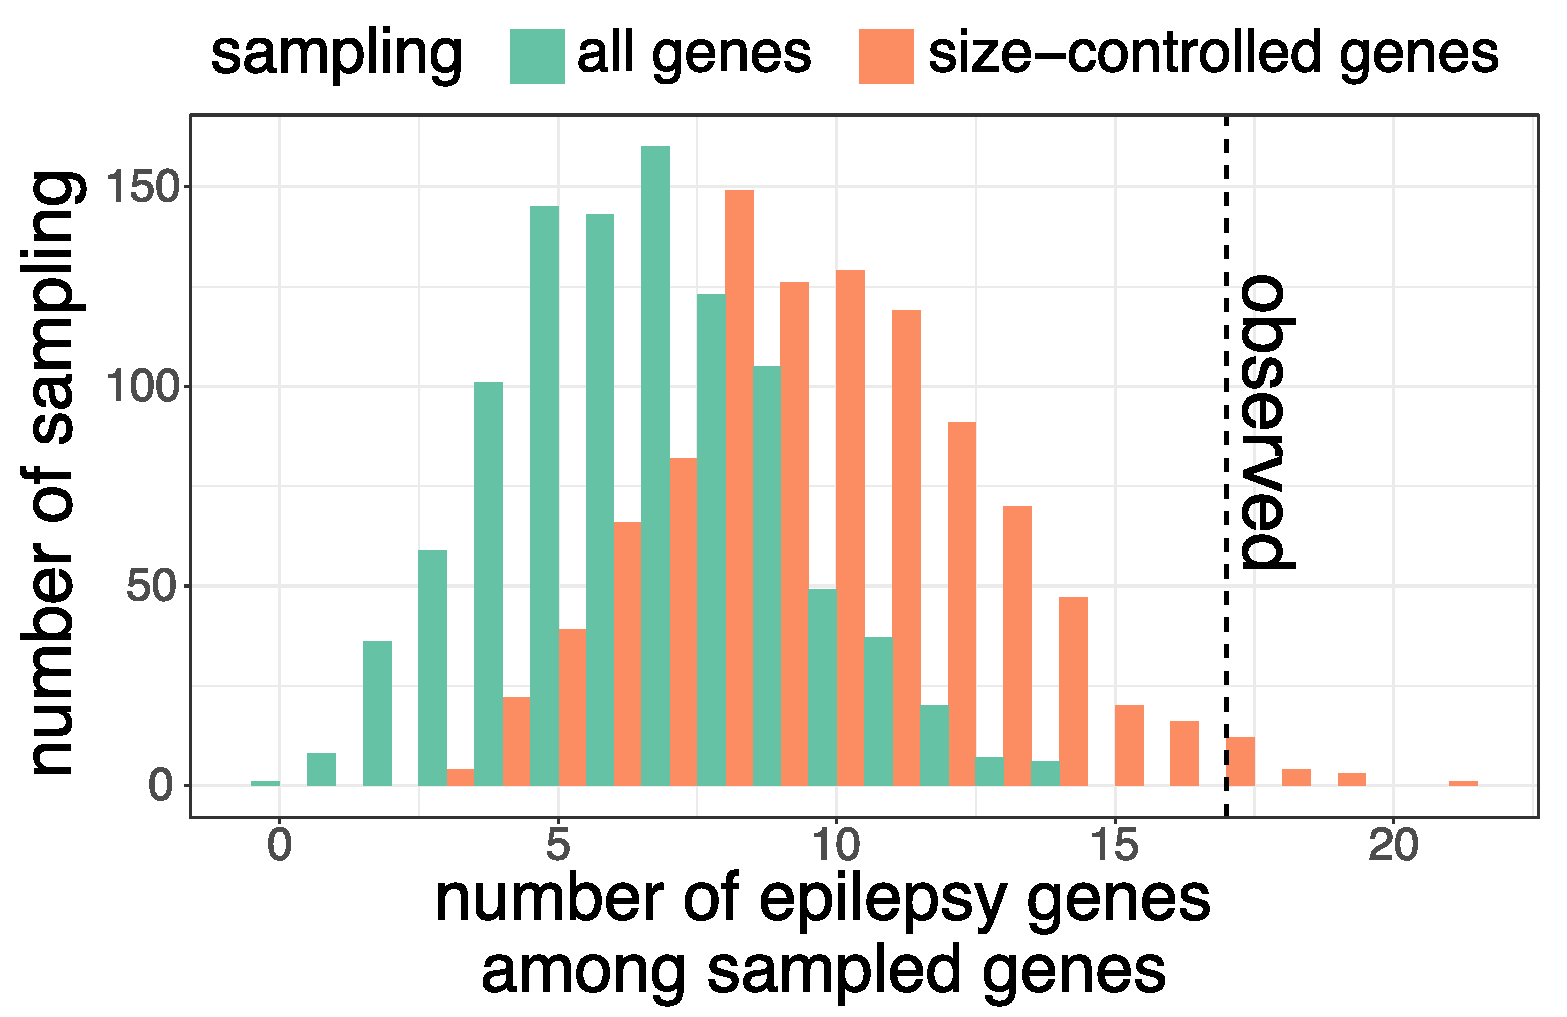
\includegraphics[width=\linewidth,page=1]{figures/epilepsy-enrichmentPatterns-long.pdf}
    \caption{}
    \label{fig:epicnvexex}
  \end{subfigure}
  
  \begin{subfigure}[b]{.9\textwidth}
    \includegraphics[width=\linewidth, page=8]{figures/epilepsy-enrichmentPatterns.pdf}
    \caption{}
    \label{fig:epidistncfun}
  \end{subfigure}
  \caption[CNVs and epilepsy genes.]{{\bf CNVs and epilepsy genes.} {\small a) Number of rare CNVs in or close to exons of protein-coding genes (top) or epilepsy genes (bottom), in the epilepsy cohort. b) Number of epilepsy genes hit by exonic deletions in the epilepsy cohort and never seen in the public and internal databases (dotted line), compared to the expected distribution in all genes and size-matched genes (histograms). c) Rare non-coding CNVs in functional regions near epilepsy genes. The graph shows the cumulative number of individuals (y-axis) with a rare non-coding CNV located at X Kbp or less (x-axis) from the exonic sequence of a known epilepsy gene. We used CNVs overlapping regions functionally associated with the epilepsy gene (eQTL or promoter-associated DNase site).}}
\end{figure}


To get a better idea of the functional regions close to epilepsy genes, we retrieved their associated eQTLs in the GTEx database\cite{Ardlie2015} and the DNase hypersensitivity sites associated with their promoter regions\cite{Maurano2012}.
Notably, focusing on rare non-coding CNVs overlapping these functional regions, the enrichment in epileptic patients was greatly strengthened and clearly present up to 100 Kbp from an epilepsy gene (Kolmogorov-Smirnov test: P-value $9\times10^{-5}$, Fig. \ref{fig:epidistncfun}).
Comparing epilepsy patients and controls, the odds ratio of having such a CNV at a distance of 100 Kbp or less from an exon was 1.33 and gradually increased the closer to the exon (2.9 for CNVs at 5 Kbp or less, Fig. \ref{fig:epidistncfunOR}).
These non-coding CNVs were rare even in the epileptic cohort, but collectively represented an important fraction of affected patients.
While 20 patients (10.1\%) had exonic CNVs in epilepsy genes that were not seen in any control or in the public and internal databases, this number rose to 57 patients (28.8\%) when counting non-coding CNVs in functional regions located at less than 100 Kbp of an epilepsy gene. %71 epilepsy genes were affected across the 92 patients.
These non-coding CNVs were never seen in the controls nor the CNV databases and overlap with annotated enhancer of epilepsy genes.
Although their functional impact remains putative, we believe these CNVs to be of high-interest for the identification of disease causing genes.
Among these CNVs of high-interest, a duplication of a regulatory region 5 Kbp downstream of {\it CSNK1E} was detected and validated in two different patients but absent from our controls and the public and internal databases (Fig. \ref{fig:ncepiex1}).
Another example is a short deletion of an extremely conserved region downstream of {\it FAM63B}, detected in one patient and overlapping expression QTLs for this epilepsy gene (Fig. \ref{fig:ncepiex2}).

\subsection*{Putatively pathogenic CNVs}
Next, we used an array of criteria to select the rare CNVs (less than 1\% in 301 controls) with the highest disruptive potential in the epilepsy cohort.
Priority was given to exonic CNVs in genes already known to be associated with epilepsy.
For CNVs in other genes, we also prioritize recurrent variants and deletions in genes highly intolerant to loss-of-function mutations.
In total, we identified 21 such putative pathogenic CNVs (Tables \ref{tab:1}-\ref{tab:2} and Table \ref{tab:supp}).
Out of these, 8 directly affected a gene previously associated with epilepsy\cite{Ran2015} (Table \ref{tab:1}).
In particular, we identified a deletion resulting in the loss of more than half of the \textit{DEPDC5} gene in a patient affected with partial epilepsy.
A number of point mutations have previously been reported in this gene for the same condition\cite{Dibbens2013,Ishida2013}.
We also identified two deletions and one duplication in \textit{CHD2} gene (see Fig. \ref{fig:popsvCHD2}).
The first deletion is large and affects a major portion of the gene while the second is a small 4.6 Kbp deletion of exon 13, the last exon of {\it CHD2}'s second isoform (Fig. \ref{fig:chd213}).
No exon-disruptive CNVs were reported in any individuals from the control cohort.
This gene was previously associated with patients suffering from photosensitive epilepsy\cite{Galizia2015}.
Interestingly, all three patients carrying the CNVs in \textit{CHD2} have been diagnosed with eyelid myoclonia epilepsy with absence, the same diagnosis that was largely enriched in the Galizia \textit{et al.} study.
Other known epilepsy genes affected by deletions include \textit{LGI1} and the 15q13.3 region.

\begin{figure}[!h]
  \centering
  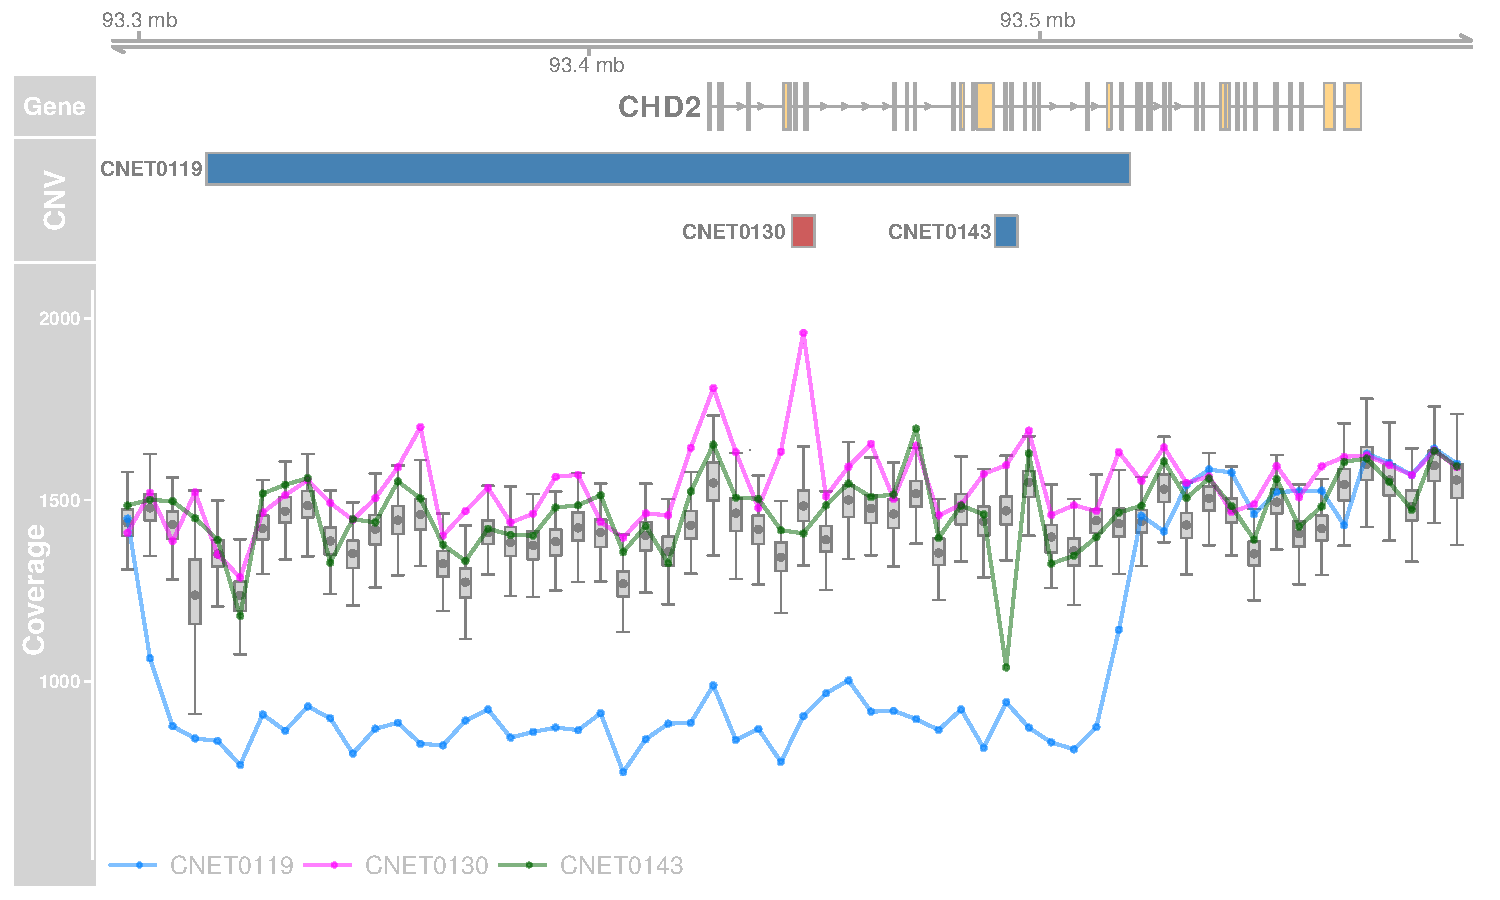
\includegraphics[width=.8\linewidth, page=1]{figures/EpiPopSV-example.pdf}
  \caption[Exonic CNVs in {\it CHD2} detected by {\sf PopSV}.]{{\bf Exonic CNVs in {\it CHD2} detected by {\sf PopSV}.} {\small The 'CNV' panel shows the exonic deletions (blue) and duplications (red) called by {\sf PopSV}. The 'Coverage' panel shows the read depth signal in the affected individuals (colored points/lines) and the coverage distribution in the reference samples (boxplot and grey point).}}
  \label{fig:popsvCHD2}
\end{figure}

\begin{table}[!ht]
  \centering
  \caption[Pathogenic profiles in known epilepsy genes.]{{\bf Pathogenic profiles in known epilepsy genes.}}
  % \begin{tabular}{|l|l|l|r|r|r|p{.2\textwidth}|r|l|l|l|l|l|}
  \resizebox{\textwidth}{!}{
    \begin{tabular}{|l|l|p{.3\textwidth}|l|l|l|l|l|l|l|l|l|l|}
      \hline
      \multirow{2}{*}{{\bf Patient  }} & \multirow{2}{*}{{\bf Epilepsy type }} & \multirow{2}{*}{{\bf Syndrome}} &  {\bf Copy}  & \multirow{2}{*}{{\bf Chr. }} & \multirow{2}{*}{{ \bf CNV start }} & \multirow{2}{*}{{ \bf CNV end   }} & { \bf Epilepsy gene with } & \multirow{2}{*}{{ \bf Taqman probe   }} & \multicolumn{2}{c|}{{\bf Discovery} } & \multicolumn{2}{c|}{{\bf Replication}} \\

                                       &             &                                         & {\bf number} &                     &           &           & {\bf exon disrupted}  &                 & {\bf Patients  } & {\bf Controls } & {\bf Patients     } & {\bf Controls    } \\
      \hline
      CNET0108   & Generalized & Eyelid myoclonia epilepsy with absence  & 1            & 1                   & 44195001  & 44460000  & {\it ST3GAL3}               & Hs05759463\_cn  & 1 DEL            & 0               & 0                   & -                  \\
      \hline
      CNET0159 & Generalized & Eyelid myoclonia epilepsy with absence  & 1            & 8                   & 141925001 & 142010000 & {\it PTK2}                 & Hs06202928\_cn  & 1 DEL            & 0               & 0                   & -                  \\
      \hline
      CNET0093 & Generalized & Juvenile onset; GTCs, Abs, Comp Partial & 1            & 10                  & 95525001  & 95545000  & {\it LGI1}                 & Hs02682696\_cn  & 1 DEL            & 0               & 0                   & -                  \\
      \hline
      CNET0140 & Generalized & Idiopathic generalized epilepsies       & 1            & 13                  & 35750001  & 35785000  & {\it NBEA}                  & Hs05286691\_cn  & 1 DEL            & 0               & 0                   & -                  \\
      \hline
      CNET0144 & Generalized & Eyelid myoclonia epilepsy with absence  & 1            & 15                  & 22745001  & 23275000  & {\it NIPA2}                 & Hs04452887\_cn  & 3 DEL            & 2 DEL           & 4 DEL (2DUP)        & 1 DEL (5 DUP)      \\
      \hline
      CNET0009 & Generalized & Idiopathic generalized epilepsies       & 1            & 15                  & 30910001  & 32445000  & {\it CHRNA7}                & Hs03909657\_cn  & 1 DEL            & 0               & 3 DEL               & (1 DUP)            \\
      \hline
      CNET0119 & Generalized & Eyelid myoclonia epilepsy with absence  & 1            & \multirow{3}{*}{15} & 93300001  & 93515000  & \multirow{3}{*}{{\it CHD2}} & Hs05385106\_cn  & 1 DEL            & 0               & 0                   & -                  \\
      CNET0143 & Generalized & Childhood absence epilepsy              & 1            &                     & 93489776  & 93494317  &                       & Hs026436998\_cn & 1 DEL            & 0               & 0                   & -                  \\
      CNET0130 & Generalized & Eyelid myoclonia epilepsy with absence  & 3            &                     & 93445001  & 93450000  &                       & Hs01379802\_cn  & 1 DUP            & 0               & 0                   & -                  \\
      \hline
      CNET0074 & Focal       & Frontal Lobe  Epilepsy                  & 1            & 22                  & 32125001  & 32255000  & {\it DEPDC5}                & Hs01632214\_cn  & 1 DEL            & 0               & 0                   & -                  \\
      \hline
    \end{tabular}
  }
  \begin{flushleft}
    The 198 epileptic patients and 301 controls represent the discovery set. The replication set contains 325 epileptic patients and 380 controls. Variants that were not tested are marked with ``-''.
  \end{flushleft}
  \label{tab:1}
\end{table}


Four of the 21 putative pathogenic CNVs were found in more than one individual (see Table \ref{tab:2} for precise numbers).
To assess their global prevalence we tested them in an additional cohort of 325 epileptic patients and 380 ethnically matched controls (Table \ref{tab:2}).
Two regions were replicated: the first region in chromosome 2 consists of duplication of the genes \textit{TTC27}, \textit{LTBP1} and \textit{BIRC6}.
In total, 4 patients carried this duplication and it was not reported in any of the two sets of controls.
The second region was found on chromosome 16 and encompasses several genes.
Two deletions were found in epileptic patients for this region and 1 epileptic individual and 1 control were also carriers of a duplication in the same region.
This region corresponds to a genomic hotspot whose deletions were previously associated with epilepsy\cite{Mefford2010} and other neurological disorders.
Finally, the remaining putative pathogenic CNVs were also associated with a number of genes (see Table \ref{tab:supp}).
However, as we lack additional evidence for those specific CNV regions, we propose that these genes should be assessed in independent epilepsy cohorts.
Of note, one patient had a rare 170 Kbp deletion encompassing three exons of the \textit{PTPRD} gene which is predicted to be highly intolerant to loss-of-function mutations (pLI=1)\cite{Lek2016}.
Rare deletions in this gene were previously found in four independent individuals with attention-deficit hyperactivity disorder\cite{Elia2010} and associated with intellectual disability\cite{Choucair2015}.
In addition, {\it de novo} deletions were found in an individual with autism\cite{Pinto2010} and more recently in a patient with epileptic encephalopathy\cite{Mefford2015}.
A common intronic variant in {\it PTPRD} was also associated with remission of seizures after treatment in a clinical cohort of epilepsy patients\cite{Speed2014a}.

\begin{table}[!ht]
  \centering
  \caption[Recurrent CNVs with a pathogenic profile.]{{\bf Recurrent CNVs with a pathogenic profile.}}
  \resizebox{\textwidth}{!}{
    \begin{tabular}{|l|l|p{.3\textwidth}|l|l|l|l|p{.3\textwidth}|l|l|l|l|l|}
      \hline
      \multirow{2}{*}{{\bf Patient}} & \multirow{2}{*}{{\bf Epilepsy type}} & \multirow{2}{*}{{\bf Syndrome }}       & {\bf Copy }  & \multirow{2}{*}{{\bf Chr. }} & \multirow{2}{*}{{\bf CNV start }} & \multirow{2}{*}{{\bf CNV end}} & {\bf Gene with}                                                & \multirow{2}{*}{{\bf Taqman probe }} & \multicolumn{2}{c|}{{\bf Discovery}} & \multicolumn{2}{c|}{{\bf Replication}}                                     \\
                                     &                                      &                                        & {\bf number} &                              &                                   &                                & {\bf exon disrupted}                                           &                                      & {\bf Patients}                       & {\bf Controls}         & {\bf Patients}           & {\bf Controls}         \\
      \hline
      CNET0184                        & Generalized                          & Lennox-Gastaut syndrome                & 3            & \multirow{2}{*}{2}           & \multirow{2}{*}{32625001}         & \multirow{2}{*}{33335000}      & \multirow{2}{*}{{\it TTC27};{\it LTBP1};{\it BIRC6}}                       & \multirow{2}{*}{Hs03387774\_cn}      & \multirow{2}{*}{2 DUP}               & \multirow{2}{*}{0}     & \multirow{2}{*}{2 DUP}   & \multirow{2}{*}{0}     \\
      %% \hline
      CNET0097                        & Generalized                          & Eyelid myoclonia epilepsy with absence & 3            &                              &                                   &                                &                                                                &                                      &                                      &                        &                          &                        \\
      \hline
      CNET0020                        & Generalized                          & Juvenile myoclonic epilepsy            & 1            & \multirow{2}{*}{12}          & \multirow{2}{*}{7995001}          & \multirow{2}{*}{8125000}       & \multirow{2}{*}{{\it SLC2A3};{\it SLC2A14}}                                & \multirow{2}{*}{Hs04406005\_cn}      & \multirow{2}{*}{2 DEL}               & \multirow{2}{*}{2 DEL} & \multirow{2}{*}{2 DEL}   & \multirow{2}{*}{2 DEL} \\
      %% \hline
      CNET0198                        & Focal                                & Frontal lobe epilepsy                  & 1            &                              &                                   &                                &                                                                &                                      &                                      &                        &                          &                        \\
      \hline
      CNET0012                        & Generalized                          & Idiopathic generalized epilepsy        & 3            & \multirow{2}{*}{15}          & \multirow{2}{*}{90845001}         & \multirow{2}{*}{90955000}      & \multirow{2}{*}{{\it ZNF774};{\it IQGAP1}}                                 & \multirow{2}{*}{Hs03895490\_cn}      & \multirow{2}{*}{2 DUP}               & \multirow{2}{*}{0}     & \multirow{2}{*}{(1 DEL)} & \multirow{2}{*}{0}     \\
      %% \hline
      CNET0167                        & Generalized                          & Childhood absence epilepsy             & 3            &                              &                                   &                                &                                                                &                                      &                                      &                        &                          &                        \\
      \hline
      CNET0063                        & Generalized                          & Idiopathic generalized epilepsies      & 3            & \multirow{2}{*}{16}          & \multirow{2}{*}{15460001}         & \multirow{2}{*}{16290000}      & {\it KIAA0430};{\it MPV17L}; {\it NPIPA5};{\it C16orf45}; {\it ABCC6};{\it NDE1}; {\it FOPNL};{\it ABCC1};{\it MYH11} & \multirow{2}{*}{Hs05396556\_cn}      & \multirow{2}{*}{1 DUP + 1 DEL}       & \multirow{2}{*}{0}     & \multirow{2}{*}{1 DEL}   & \multirow{2}{*}{1 DUP} \\
      %% \hline
      CNET0037                        & Generalized                          & Idiopathic generalized epilepsies      & 1            &                              &                                   &                                &                                                                &                                      &                                      &                        &                          &                        \\
      \hline
    \end{tabular}
  }
  \begin{flushleft}
    The 198 epileptic patients and 301 controls represent the discovery set. The replication set contains 325 epileptic patients and 380 controls.
  \end{flushleft}
  \label{tab:2}
\end{table}


\section{Discussion}

Although several tools exist for the detection of CNVs using WGS data, we found that none of them could efficiently account for technical biases, thus resulting in limited sensitivity.
To improve on this, we developed a new tool, {\sf PopSV}, which we demonstrated was able to accurately detect CNVs, including rare and small events.

%% Importance of the reference samples
A key aspect of our approach is the use of a set of reference samples to identify abnormal read coverage.
In this context, the choice and number of reference samples will have an effect on the analysis.
Results from running {\sf PopSV} using different reference cohort sizes suggest that CNV calls are consistent across runs but that a higher number of reference samples increases the sensitivity and robustness of the CNV detection (Fig. \ref{fig:cohortsize}).
Based on these results, we recommend {\sf PopSV} when 20 samples or more can be used as reference.
In a given study, all samples can be used as a reference, or a subset of a few hundreds if the total sample size is extremely large.
Although variants with frequency around 50\% might not be detected, {\sf PopSV} excels at detecting less frequent variants, smaller variants or variants in challenging regions such as repeat-rich regions.
In a case/control design, the control samples could be used as reference in order to maximize the detection of case-specific variants.
In the current study we used both epilepsy patients and controls as reference in order to be able to directly compare the observed CNV distributions.
Finally, in a cancer project with paired normal and tumor samples, only normal samples should be used as reference such that {\sf PopSV} can detect somatic CNVs of any frequency.

%% Importance of same processing. Mention aligner.
To maximize performance, the same library preparation, sequencing and data pre-processing should be employed on all the samples.
To identify potential batch effects, a principal component analysis of read coverage was implemented as part of the {\sf PopSV} package and is recommended to assess the homogeneity of the reference samples.
The read length and aligner can lead to drastic changes in the read coverage and should be consistent across the cohort when analyzed with {\sf PopSV}.
This is particularly important in repeat-rich regions.
Although the different datasets were produced by different sequencing and pre-processing protocols and showed varying degrees of technical bias (Fig. \ref{fig:wgsbias}, \ref{fig:bias:varrank} and \ref{fig:wgsbias2}), the performance of {\sf PopSV} was comparable when benchmarking the methods in the two public datasets and experimentally validating calls in the CENet cohort.

%% Extensions
%% Exome extension
{\sf PopSV}'s approach does not require a uniform read coverage and integrate the coverage variation separately in each studied region.
For these reasons, it would be straightforward to analyze targeted sequencing data, such as exome-sequencing.
%% SV extension
{\sf PopSV} could also be extended for the detection of other types of SVs such as balanced SVs.
To do this, instead of counting properly mapped reads, the method could be modified to test for an excess of discordant reads.
%% Copy-number estimation and breakpoint resolution.
Finally, additional modules could be added to {\sf PopSV} to help characterize the detected variants.
For instance, instead of computing a copy-number estimate from the average coverage in the reference, a HMM approach including all samples could provide a better genotyping strategy.
Similar to other approaches\cite{Abyzov2011,Benjamini2012}, an additional step in the pipeline could explore the effect of the bin size on the variation in read coverage across the population and suggest an optimal bin size.

As in previous array-based studies\cite{Mefford2011,Heinzen2010,Striano2012}, we observed an enrichment of large rare exonic CNVs in patients compared to controls.
However, thanks to the resolution of WGS and {\sf PopSV}, we found that the global distribution of small CNVs ($<$50 Kbp) in 198 unrelated epilepsy patients was also skewed towards rare exonic CNVs.
In addition, genes disrupted by rare deletions in patients were enriched for previously known epilepsy genes.
These observations support the association of small CNVs with epilepsy and could not have been detected in previous array-based studies.

We also observed a clear enrichment of non-coding CNVs in the neighborhood of previously implicated genes.
When focusing on CNVs seen only in the epilepsy cohort and around epilepsy genes, 10.1\% of epilepsy patients have an exonic CNVs and our results shows that up to 28.8\% of patients harbor non-coding CNVs of high-interest in the proximity of epilepsy genes.
These non-coding variants are present in the epilepsy cohort only and located in annotated regulatory regions associated to known epilepsy genes.
Although it is challenging to directly test their functional impact, their frequency and location suggest a putative importance in the genetic mechanism of epilepsy and should be further investigated in the future.

Finally, to better understand the impact of these findings on an individual scale, we selected CNVs with the highest pathogenic potential within our patients.
These CNVs highlighted known but also potentially new epilepsy genes.
Using a second epilepsy cohort, we were also able to identify two chromosomal regions that were recurrently disrupted by CNVs.
These findings highlight the benefits of having a comprehensive survey of CNVs when trying to understand the genetic causes of a disease.


\section{Materials and Methods}

\subsection*{Ethics Statement}
This study was approved by the Research Ethics Board at the Sick Kids Hospital (REB number \verb!1000033784!) and the ethics committee at the Centre Hospitalier Universitaire de Montr\'eal (project number \verb!2003-1394,ND02.058-BSP(CA)!).
Before their inclusion in this study, patients or parents (when needed) had to give written informed consents.

\subsection*{Epilepsy patients and sequencing}
Patients were recruited through two main recruitment sites at the Centre Hospitalier Universitaire de Montr\'eal (CHUM) and the Sick Kids Hospital in Toronto as part of the Canadian Epilepsy Network (CENet).
The main cohort of this study was constituted of 198 unrelated patients with various types of epilepsy; 85 males and 113 females.
The mean age at onset of the disease for our cohort was 9.2 ($\pm$6.7) years.
Table \ref{tab:clinical} presents a detailed description of the clinical features for the various individuals recruited in this study.
301 unrelated healthy parents of other probands from CENet were also included in this study and used as a control cohort.
DNA was exclusively extracted from blood DNA.

Libraries were generated using the TruSeq DNA PCR-Free Library Preparation Kit (Illumina) and paired-end reads of size 125 bp were sequenced on a HiSeq 2500 to an average coverage of 37.6x $\pm$ 5.6x.
Reads were aligned to reference Homo\_sapiens b37 with {\sf BWA}\cite{Li2010}.
Finally, Picard was used to merge, realign and mark duplicate reads.
Raw sequence data has been deposited in the European Genome-phenome Archive, under the accession code \href{https://www.ebi.ac.uk/ega/studies/EGAS00001002825}{EGAS00001002825}.
For more details, see \nameref{sec:suppmat:epipopsv}.

\subsection*{Public WGS datasets}
Two high-coverage public datasets were used to benchmark {\sf PopSV} against existing methods.

A {\it Twin} study provided WGS sequencing data for 45 individuals, including 10 monozygotic twin quartets from the Quebec Study of Newborn Twins\cite{Boivin2013}.
All patients gave informed consent in written form to participate in the Quebec Study of Newborn Twins. Ethic boards from the Centre de Recherche du CHUM, from the Universit\'e Laval and from the Montreal Neurological Institute approved this study.
DNA was extracted from blood and sequencing was done on an Illumina HiSeq 2500 (paired-end mode, fragment length ~300 bp).
The reads were aligned using a modified version of the Burrows-Wheeler Aligner\cite{Li2010} (bwa version 0.6.2-r126-tpx with threading enabled).
The options were \verb!'bwa aln -t 12 -q 5' and 'bwa sampe -t 12'!.
Aligned reads are available on the European Nucleotide Archive under ENA \href{https://www.ebi.ac.uk/ena/data/view/PRJEB8308}{PRJEB8308}.
The 45 samples had an average sequencing depth of 40x (minimum 34x / maximum 57x).

A cancer dataset from a study of renal cell carcinoma\cite{Scelo2014} was also used.
95 pairs of normal/tumor tissues were sequenced using GAIIx and HiSeq2000 instruments.
Paired-end reads of size 100 bp totaled an average sequencing depth of 54x (minimum 26x / maximum 164x).
Reads were trimmed with FASTX-Toolkit and mapped per lane with {\sf BWA}\cite{Li2010} backtrack to the GRCh37 reference genome.
Picard was used to adjust pairs coordinates, flag duplicates and merge lanes.
Finally, realignment was done with {\sf GATK}.
Raw sequence data has been deposited in the European Genome-phenome Archive, under the accession code \href{https://www.ebi.ac.uk/ega/studies/EGAS00001000083}{EGAS00001000083}.
More details can be found in Scelo et al.\cite{Scelo2014}.

\subsection*{Testing for technical biases in WGS}
To investigate the bias in read depth (RD), we fragmented the genome in non-overlapping bins of 5 Kbp and counted the number of properly mapped reads. 
In each sample, we corrected for GC bias and removed bins with extremely low or high coverage (see \nameref{sec:suppmat:epipopsv}). 
Then, read counts across all samples were combined and quantile-normalized. 
Using simulations and permutations, we constructed two control RD datasets with no region-specific or sample-specific bias. 
We computed the mean and standard deviation of the coverage in each bin across samples. 
Next, to investigate experiment-specific bias, we retrieved which sample had the highest coverage in each bin. 
Then we computed, for each sample, the proportion of the genome where it had the highest coverage. 
The same analysis was performed monitoring the lowest coverage. 
This analysis was performed separately on the CENet dataset, the Twin dataset and the normal samples from the cancer dataset.
On the Twin dataset, the same analysis was also run after correcting the read coverage following the {\sf QDNAseq} pipeline\cite{Scheinin2014} (see \nameref{sec:suppmat:epipopsv}).

\subsection*{{\sf PopSV}}
The main idea behind {\sf PopSV} is to assess whether the coverage observed in a given location of the genome diverges significantly from the coverage observed in a set of reference samples.
{\sf PopSV} was implemented in an R package (see \nameref{sec:code}).
The genome is first segmented into bins and the number of reads with proper mapping in each bin is counted for each sample.
In a typical design, the genome is segmented in non-overlapping consecutive windows of equal size, but custom designs could also be used.
With {\sf PopSV}, we propose a new normalization procedure which we call targeted normalization that retrieves, for each bin, other genomic regions with similar profile across the reference samples and uses these bins to normalize read coverage (see \nameref{sec:suppmat:epipopsv}).
Our targeted normalization was compared to global approaches that adjust for the median coverage, or quantile-based approaches.
After normalization, the value observed in each bin is compared with the profiles observed in the reference samples and a Z-score is calculated (Fig. \ref{fig:popsv}).
False Discovery Rate (FDR) is estimated based on these Z-score distributions and a bin is marked as abnormal based on a user-defined FDR threshold.
Consecutive abnormal bins are merged and considered as one variant.
In {\sf PopSV}'s R package, circular binary segmentation\cite{Seshan2017} can also be used to merge bins into variant regions.
Copy number was estimated by dividing the coverage in a region by the average coverage across the reference samples, multiplied by 2 (see \nameref{sec:suppmat:epipopsv}).

\subsection*{Validation and benchmark of {\sf PopSV}}
We compared {\sf PopSV} to {\sf CNVnator}\cite{Abyzov2011}, {\sf FREEC}\cite{Boeva2011} and {\sf cn.MOPS}\cite{Klambauer2012}, three popular RD methods that can be applied to WGS datasets.
We also ran {\sf LUMPY}\cite{Layer2012} which uses an orthogonal mapping signal: the insert size, orientation and split mapping of paired reads. For {\sf LUMPY}, all the CNVs (deletions and duplications) and intra-chromosomal translocations (labeled as 'BND' in Lumpy's output) larger than 300 bp were kept for the upcoming analysis.
These methods were run on the two publicly available datasets, using 5 Kbp bins for the RD methods.

First, we compared the frequency at which a region is affected by a CNV using the calls from the different methods.
To investigate the presence of systematic calls in each method, we compute how many of the calls in a typical sample are called at different frequencies in the dataset.
For example, on average, how many calls in one sample are called in more than 90\% of the samples.
In the Twin dataset, the samples were clustered using the CNV calls from each method.
Different linkage criteria were used for the hierarchical clustering (see \nameref{sec:suppmat:epipopsv}).
The Rand index estimated the concordance between the clustering and the known pedigree (family-level).
Next, we measured the number of CNVs identified in each twin that were also found in their monozygotic twin.
We removed calls present in more than 50\% of the samples to ensure that systematic errors were not biasing our replication estimates.
Hence, a replicated call is most likely true as it is present in a minority of samples but consistently in the twin pair.
For {\sf CNVnator}, {\sf LUMPY} and {\sf PopSV}, the eval1/eval2 columns, number of supporting reads and adjusted P-values (respectively) were used to gradually filter low-quality calls and explore their effect on the replication metrics.
In addition to their replication, we annotated the calls when their region overlapped a call found by other methods in the same sample.
For calls found by at least two methods, we computed the proportion of calls from a method found by each of the other methods.

The approach described previously comparing pairs of twins was also applied in the cancer dataset, on pairs of normal/tumor samples.
In this case, a replicated call is found in the normal sample and in the paired tumor sample.
Finally, we compared calls using small bins (500 bp) and calls using larger bins (5 Kbp).
This comparison explores the quality of the calls, the size of detectable events and the resolution for different bin sizes.
First, we counted how many small bin calls supported any large bin call.
We then looked at the proportion of small bin calls of different sizes that were also found in the large bin calls.

\subsection*{CNV detection in the CENet cohorts}
CNVs were called using {\sf PopSV} using 5 Kbp bins and all the samples from both the epilepsy and control cohorts as reference.
We annotated the frequency of the CNVs using germline CNV calls from the Twin and cancer datasets (internal database) as well as four public CNV databases from the 1000 Genomes Project\cite{Sudmant2015a,Handsaker2015}, the Genome of Netherlands\cite{Francioli2014} and the Simons Genome Diversity Project\cite{Sudmant2015}.
CNVs were annotated with the maximum frequency in the databases.
Hence, a rare CNV is defined as present in less than 1\% of the samples in each of the five CNV databases.

To test for a difference in deletion/duplication ratio among rare CNVs, we compared the numbers of rare deletions and duplications in the epilepsy patients and controls using a $\chi^2$ test.
The same test was performed after downsampling the controls to the sample size of the epilepsy cohort.

\subsection*{Validation by Taqman RT-PCR}
We first selected CNV calls in epilepsy patients that spanned at least 2 consecutive bins.
We kept exonic CNVs of different sizes and overlapping a Taqman probe.
A second batch of CNVs, containing small non-coding CNVs, was also sent for validation.
Here, hundreds of non-coding CNVs spanning only one bin were randomly selected.
When possible the breakpoints were manually fine-tuned from manual inspection of a base-pair level coverage representation or using {\sf IGV}\cite{Thorvaldsdottir2013}; the breakpoints remained unchanged when they could not be refined.
Finally, we kept regions overlapping a Taqman probe.

Probes were selected using the assay search tool on the Thermofisher website.
All probes were tested for patients and controls that were called in {\sf PopSV} as well as an additional 10 control individuals to ensure the validity of the probe.
For each CNV, one assay was chosen in the middle of the genomic region of interest and located in an exon when possible.
All reactions with TaqMan Copy Number Assays were performed in duplex using the FAM dye label based assay for the target of interest (Taqman copy number assay, Made to order, \#4400291, Applied Biosystems by Life Technologies) and the VIC dye label based TaqMan Copy Number Reference Assay for RNase P (4403326, Life technologies).
Amplification reactions ($10\mu L$), which were performed in quadruplicate, consisted of: 10 ng gDNA, 1X TaqMan Copy Number Assay, 1X TaqMan Copy Number Reference Assay, RNase P, 1X TaqMan Genotyping Master Mix (4371355, Life Technologies) or 1X SensiFAST Probe Lo-ROX Kit (BIO-84020, Froggabio).
PCR was performed with an Applied Biosystems QuantStudio7 flex Real-Time PCR system using the standard curve settings and the default universal cycling conditions: 95 $^{\circ}$C 10 minutes followed by 40 cycles: 95 $^{\circ}$C 15 seconds, 60 $^{\circ}$C 60 seconds.
Data was analyzed with QuantStudio Real-Time PCR system software v1.2 (Applied Biosystems by Life Technologies) using autobaseline and manual Ct threshold of 0.2.
Results export files were opened in CopyCaller\textsuperscript{TM} Software v2.0 for sample copy number analysis by the relative quantitation method.
The median $\Delta$Ct was used as the calibrator sample in the analysis settings.

\subsection*{CNV enrichment in exonic regions}
For each cohort (epilepsy and control), we retrieved the CNV catalog by merging CNV that are recurrent in multiple samples.
Hence, the CNV catalog represents all the different CNVs found in each cohort.
Because the epilepsy and control cohorts have different sample sizes, the CNV catalogs for each cohort were built using 150 randomly selected samples.
For each sub-sampling and each cohort, control regions were selected to fit the size distribution of the CNV catalog and the overlap with centromeres, telomeres and assembly gaps (see \nameref{sec:suppmat:epipopsv}).
The fold-enrichment represents how much more/less of the CNVs overlap an exon compared to the control regions.
To robustly compare the two cohorts, we computed the median difference in fold-enrichment between the CNV catalogs from patients and controls across 100 sub-sampled catalogs.
The cohort labels of the CNV catalogs were then permuted 10,000 times and the analysis repeated to derive a null distribution for the median difference in fold enrichment.
A permuted P-value was computed from the observed difference and the null distribution.

Small ($<$50Kbp) and large ($>$50 Kbp) CNVs were analyzed separately.
Exons from genes predicted to be loss-of-function intolerant\cite{Lek2016} (probability of loss-of-function intolerance $>$ 0.9) were also analyzed separately.
The same analysis was repeated using only rare CNVs, i.e. being present in less than 1\% of {\sf PopSV} calls in the Twins and renal cancer datasets, and in four public datasets (see \nameref{sec:suppmat:epipopsv}).

In each cohort, we then retrieved the CNV catalog of rare exonic CNVs.
We evaluated the proportion of the CNVs in the catalog that are private (i.e. seen in only one sample).
The control cohort was down-sampled a thousand times to the same sample size as the epilepsy cohort to provide a confidence interval and empirical P-value (see \nameref{sec:suppmat:epipopsv}).
We also visualize the proportion of CNVs in the catalog seen in 2 samples or more, 3 samples or more, etc (Fig. \ref{fig:epiexpriv}).
We performed the same analysis after removing the top 20 samples with the highest number of non-private rare exonic CNVs.
The analysis was also repeated using French-Canadian individuals only.

\subsection*{CNV enrichment in and near epilepsy genes}
We used the list of genes associated with epilepsy from the EpilepsyGene resource\cite{Ran2015} which consists of 154 genes strongly associated with epilepsy.
We tested different sets of CNVs: deletion or duplications in the epilepsy cohort, control individuals and samples from the twin study, and using different threshold of maximum frequency.
For each set of CNVs, we counted how many of the genes hit were known epilepsy genes.
To control for the size of epilepsy genes and CNV-hit genes, we randomly selected genes with sizes similar to the genes hit by CNVs and evaluated how many were epilepsy genes.
After sampling 10,000 gene sets, we computed an empirical P-value (see \nameref{sec:suppmat:epipopsv}).

To investigate rare non-coding CNVs close to known epilepsy genes, we counted how many patients have such a CNV at different thresholds of distance to the nearest exon.
We compared this cumulative distribution to the control cohort, after down-sampling it to the sample size as the epilepsy cohort.
We performed the same analysis using deletions only.
Each epilepsy gene was also tested for an excess of rare non-coding deletions in patients versus controls using a Fisher test.
Next, we restricted our analysis to rare non-coding CNVs that overlap an eQTL associated with the epilepsy genes\cite{Ardlie2015} or a DNase I hypersensitive site associated with the promoter of epilepsy genes\cite{Maurano2012}.
A Kolmogorov-Smirnov test was used to test the difference in distribution.
Finally, using different values for the maximum distance to the nearest epilepsy gene, we computed the odds ratio of having such a CNV between epilepsy patients and controls.


\subsection*{Putatively pathogenic CNVs}
Exonic CNVs larger than 10 Kbp and found in less than 1\% of the 301 controls were first selected.
We further retained either CNVs overlapping the exon of a known epilepsy-associated gene\cite{Ran2015} or deletions overlapping the exon of a loss-of-function intolerant gene\cite{Lek2016}, or CNVs present in two or more of our epilepsy patients.
All the putatively pathogenic CNVs were validated by Taqman RT-PCR.

\subsection*{Data and code availability}
\label{sec:code}

The {\sf PopSV} R package and its documentation are available at \url{http://jmonlong.github.io/PopSV/}.
Scripts are provided to run the pipeline on different high performance computing systems.
The code used for the analysis and to produce figures and numbers is documented at \url{http://github.com/jmonlong/epipopsv} and archived in \url{https://doi.org/10.5281/zenodo.1172181}.
Necessary data, including the CNV calls, was deposited at \url{https://figshare.com/s/20dfdedcc4718e465185}.
Raw sequence data has been deposited in the European Genome-phenome Archive, under the accession code \href{https://www.ebi.ac.uk/ega/studies/EGAS00001002825}{EGAS00001002825}.

\section{Acknowledgments}
Data analyses were enabled by compute and storage resources provided by Compute Canada and Calcul Qu\'ebec.
We would like to thank Pascale Marquis at the Canadian Centre for Computational Genomics for processing the raw sequencing data to genomic variant calls and for her active participation in various quality assessment steps.
The Canadian Centre for Computational Genomics (C3G) is a Node of the Canadian Genomic Innovation Network and is supported by the Canadian Government through Genome Canada.
We are grateful to the team of the Qu\'ebec Study of Newborn Twins who provided the twin dataset and the Cagekid consortium who provided the renal cancer dataset.
We would like to thank Sylvia Dobrzeniecka for sample handling and lab work.
We are grateful to Dr. Ledia Brunga for her work on the epileptic cohort and to Brianna Goldenstein and Claudia Moreau for revising this manuscript.
Finally, we would like to thank Simon Gravel, Mathieu Blanchette, Mathieu Bourgey, Toby Dylan Hocking and Claudia Moreau for helpful discussions.


%%% Local Variables:
%%% mode: latex
%%% TeX-master: "../main"
%%% End:
